\section{Problems with Local Approximations as Advice Policies}
\label{sec:linear}

One might reasonably hope that, instead of needing to bother with solving an agency MDP, a decision model's local structure can serve as a good heuristic for the incentives dictated by that model. After all, local approximation methods \cite{ribeiro2016should, baehrens2010explain} have gained widespread adoption as one of the most effective methods for interpreting otherwise-inscrutable machine learning models \cite{lundberg2016unexpected}. 

Unfortunately, even for simple non-linear decision functions, local-approximation-based advice can be dangerously wrong. We have already seen the example in Figure \ref{fig:1di}, in which a locally-improving policy would trap the individual at a local maximum and never achieve the better outcome that was available to them. Following local advice may result in individuals receiving sub-optimal decisions even when the decision function is monotonic: in Figure \ref{fig:2di} we can see that a locally-optimizing policy would lead a subject to a substantially inferior decision over the course of $6$ steps, even when each locally-optimal action seemed to improve the decision.
% Local approximation methods have become one of the primary methods for interpreting machine learning models (\citet{lundberg2016unexpected}).
% These methods are intended to identify the local structure of a function around an operating point, and use that as a proxy for its behavior in that region of the input space. These models can be computed by locally perturbing the function's input and fitting a linear model on the results (LIME, \citet{ribeiro2016should}) or, if differentiable, by computing the gradient of the function wrt. its inputs (\citet{baehrens2010explain}). 

Below, we'll lay out a definition for locally-optimal advice, and prove that it only recovers the maximally-incentivized actions for a narrow class of decision functions.

\begin{figure}
    \centering
\minipage{0.3\textwidth}
    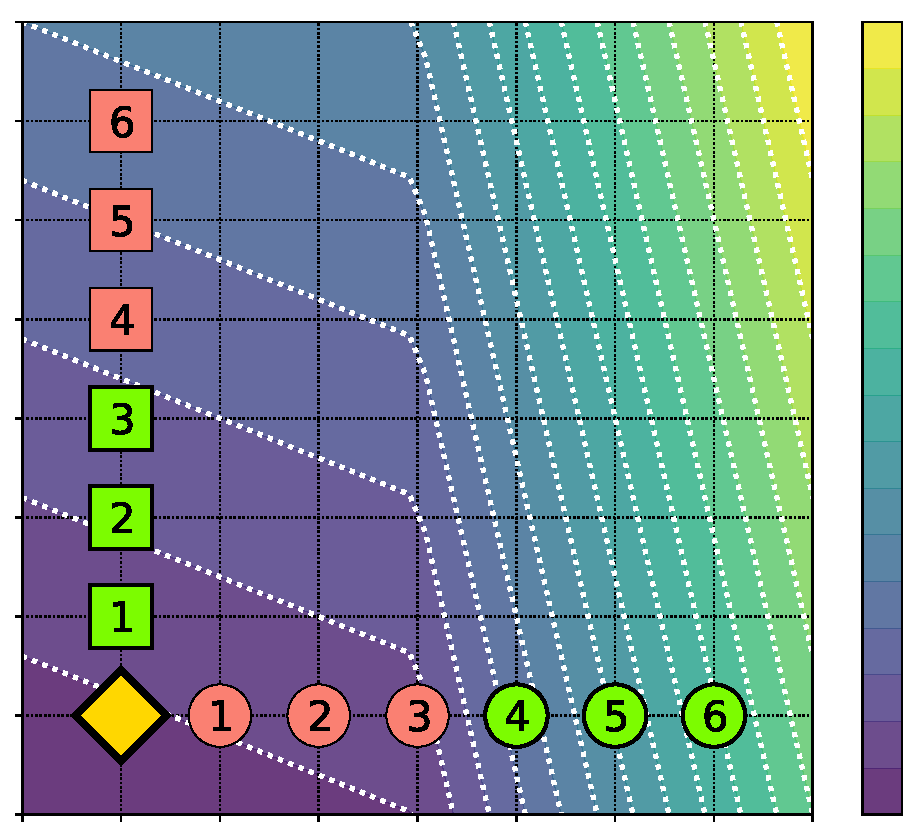
\includegraphics[width=\linewidth]{figures/incentive_2d.pdf}
\endminipage\hfill
\minipage{0.68\textwidth}
    \caption{A 2D monotonic decision function, with the lowest output in bottom-left (blue), and highest output in top-right (yellow). A subject in the bottom-left corner (gold diamond) can move $1$ grid unit each step. Circles represent the optimal agency-MDP policy given $4$ or more steps, while squares represent the greedy policy.}
\endminipage
    \label{fig:2di}
\end{figure}

%\subsection{When local approximations work, and when they fail}
\subheading{When local approximations work, and when they fail}

In our setting, we define a locally-optimal \textit{greedy} policy as a policy that chooses actions based only on maximizing the immediate improvement in the received decision:
\begin{equation}
\label{eq:greedy}
\pi_{local}(s) = \argmax_{a \in \acspace} \E_{s' \sim \tran(s,a)} \left [\dec\left(I_x(s')\right)\right ]
\end{equation}
When the function is differentiable, we can also define the \textit{gradient-following} policy for a state $s = [x, r]$ composed of only the decision features $x$ and the remaining available displacement $r$. Note that in this hypothetical transition model, we can manipulate every feature axis in $x$ independently.
\begin{equation}
\label{eq:gradient}
\pi_{gradient}(s) = \argmax_{a \in\{a' \in \RR^{dim(x)}~| ~\|a'\|_2 = \epsilon, ~\epsilon \ll 1\} } \dec(x + a) ~~= ~~ \epsilon \nabla_x\dec\left(x\right)
\end{equation}
% When the action space is the space of local feature perturbations of size $\epsilon$, i.e. $\acspace =  and $I_x(\tran(s, a)) = x + a$, then as $\epsilon \rightarrow 0$ the greedy policy becomes equivalent to stepping along the gradient: $\pi_{local}(s) \propto \nabla_x\dec(x)$. We call this advice policy \textit{gradient-following}.

% In many cases, both the gradient-following policy (and its generalized analog, the greedy policy) fail to recover optimal incentives. We have already seen the example in Figure \ref{fig:1di}, in which a greedy policy would trap the individual in a local maximum and never find the global maximum. Local incentives can lead to suboptimal behavior even when a decision function is monotonic: in Figure \ref{fig:2di} we can see that a locally-optimizing policy may lead a subject to expend unnecessary effort improving their decision, even if it would eventually reach the same result. \yocomment{Add a real-world analog?}
The following are a series of theorems about this setting; the proofs are included in Appendix \ref{sec:proofs}.
\newtheorem{theorem}{Theorem}
\begin{theorem}
\label{gradIsOptimal}
If there exists a policy that is optimal independent of the number of resources remaining, it must be equivalent to the greedy policy.
%For a policy to be optimal independent of resources remaining it must be equivalent to the greedy policy.
\end{theorem}

\newtheorem{corollary}{Corollary}[theorem]
\begin{corollary}
\label{localAreGlobal}
Only if a decision function $\dec$ satisfies the constraints required for greedy ascent to reach a global maximum from any point can the gradient-following policy be an optimal advice policy for $\dec$. This means all local maxima must also be global maxima for a decision function to have an optimial policy independent of resources.
% For a decision function $\dec$ to permit an optimal policy that does not consider resources remaining, the decision function $\dec$ must satisfy the constraints that are required for gradient descent to reach a global maximum (any local maxima are global maxima, etc).


%If a policy that is optimal independent of resources to exist for decision function $\dec$, the decision function $\dec$ must satisfy the constraints for gradient descent to work (any local maxima are global maxima, etc). \wmnote{perhaps some citations}
\end{corollary}

\newtheorem{theorem2}{Theorem}
\begin{theorem}
\label{Linear}
% For a decision function $\dec$ to permit an optimal policy that does not consider resources remaining, the gradient field of $\dec$ must consist only of straight lines whenever $\del \dec \ne 0$. \yocomment{Is this extra part necessary?} , assuming $\dec$ is not constant.

For a continuous action space in $L_2$, a greedy policy is optimal if the gradient field of $D$ consists of straight lines wherever $\del \dec \ne 0$.

\end{theorem}
\newtheorem*{remark}{Remark}

\begin{remark}
    This explains why gradient-following is not optimal in Figure \ref{fig:2di}, in spite of the function being monotonic and otherwise amenable to gradient ascent.
\end{remark}

\newtheorem{corollary2}{Corollary}[theorem2]
\begin{corollary}
\label{thm:samedirection}
For a continuous action space in $L_2$, a greedy policy is optimal only if the gradient field of $\dec$ consists of straight lines wherever $\del \dec \ne 0$.
\end{corollary}
\begin{remark}
    By Corollary \ref{thm:samedirection}, the gradient-following policy is optimal for linear and logistic regression in $L_2$.
\end{remark}


%\newtheorem{theorem3}{Theorem}
%\begin{theorem}
%\label{L1thm}
%%For a continuous action space in $L_1$, a greedy policy is optimal and independent of resources if and only if the closest optimal point requires changing at most one parameter from any starting point.
%\end{theorem}

%\begin{proof}
%Suppose we do not start on a global maximum (if we did the greedy policy should say not to move and thus is optimal and correct).
%%Consider a infinitesimal resource limit of $\epsilon$. Suppose we follow the greedy policy for a given starting point, we can define the direction $\vec{v}$ as the vector from the starting point to where we end up after $\epsilon$ resources.
%\end{proof}

%
%Moreover, consider the plane tangent to $\vec c$ at an arbitrary $x$. Gradients at all points on this plane not only must point in the same direction, but be of the same magnitude. A full proof is omitted for brevity, but intuitively if this were not the case it would be optimal a point with smaller gradient to point more in the direction a point with larger gradient and thus all gradient lines do not point in the same direction.
%
% Suppose this were not the case. Therefore there must exist an $\vec x$, $\vec x+\vec \epsilon$ on the plane such that the gradients pointed in the same direction but had different magnitudes. WLOG suppose $|\del \dec(\vec x)| > |\del \dec(\vec x+\vec \epsilon)|$ Therefore following the gradient field at $\vec x$ a distance $\d$ will result in a larger decision than that of following $\vec x + \vec \epsilon$. However, the gradient must point towards
%
% Formally, this implies that (for positive definite $g$):

% \begin{align}
%     \nabla f &= \vec{c} g(\vec x),\;\;g(\vec x) > 0 \; \forall x\\
%     \frac{\nabla_i f}{g(\vec x)} &= c_i
% \end{align}
% \yocomment{What does this second line mean? What is the constraint being placed on g? That it is decomposable?}\wmnote{The constraint is that g is positive definite (always above zero)}
%
% Suppose $\nabla_i f, c_i \ne 0$ for some $i$ (which must be the case since the function is not constant).
% \begin{align}
%     \frac{\nabla_j f}{\nabla_i f} &= \frac{c_j}{c_i},\; \forall j \\
%     \nabla_j f &= \frac{c_j}{c_i} \nabla_i f,\; \forall j\\
%     g(\vec x) &= h(\vec c \cdot \vec x)\\
%     \nabla f &= \vec{c} h(\vec{c} \cdot \vec x),\;\;h(m) > 0 \; \forall m\\
% \end{align}
% (Moved to rest to supplement.tex)
%Let us consider the conditions necessary to derive an optimal policy. 